\documentclass[../ai_in_finance]{subfiles}
\usepackage[margin=1in]{geometry}
\usepackage{tikz}
\usetikzlibrary{positioning}
\usepackage{amsmath}
\usepackage{amssymb}
\usepackage{booktabs}
\usepackage{graphicx}
\usepackage{draftwatermark}

\SetWatermarkText{WSuo@Queensu.ca}
\SetWatermarkScale{1.4}
\SetWatermarkColor{gray!35}
\SetWatermarkAngle{45}

\usepackage{makeidx}
\makeindex

\begin{document}

\chapter{Valuation and Asset Pricing}

\section{Introduction}

The preceding chapters built the pieces needed to price a financial asset: Chapter 3 described the institutions and instruments that are traded, and Chapter 4 showed how a firm's financial statements reveal the cash flows it actually generates. This chapter puts those pieces together and asks the central question of asset pricing: given a stream of future cash flows, or a payoff that depends on some other asset's price, what should that claim be worth today?

The chapter answers this question with worked numerical examples for the three main instrument classes introduced in Chapter 3: bonds, equities, and derivatives. Every formula here is accompanied by a computation a reader can check by hand or reproduce in the companion notebook, in keeping with this book's view that a quantitative finance practitioner should be able to compute a price directly, not just describe the logic behind it qualitatively.

The chapter is organized to build in complexity. It begins with the simplest possible cash flow structures, a single-maturity bond and a constant-growth dividend stream, where closed-form formulas exist and every number can be verified by hand. It then introduces two ways of estimating the discount rate that all of these formulas depend on, the term structure of interest rates and the cost of capital, before turning to the more complex, nonlinear payoffs of options, which require the replication and no-arbitrage arguments central to modern derivatives pricing. A useful way to read the chapter is as a single valuation story: Meridian Fabrication\index{Meridian Fabrication Inc.}, the running example introduced in Chapter 4, is first valued from its projected cash flows, then compared with a market-based multiple, and finally used to illustrate how a firm's financing mix determines the discount rate. The goal is not to treat bonds, equities, and options as unrelated topics, but to show that the same present-value logic reappears in each context.

\section{The Time Value of Money, Revisited}\index{Time Value of Money, Revisited}

Chapter 1 introduced the present value relation 
$$V = \sum_{t=1}^{T} \frac{CF_t}{(1+r)^t}$$ 
as the unifying idea behind bond pricing, stock valuation, and project appraisal. This chapter makes that idea operational. Two quantities determine the value of any claim on future cash flows: the size and timing of the cash flows themselves, and the discount rate $r$, which compensates the holder for the time value of money and for the risk that the cash flows might not arrive as expected. A safer stream of cash flows is discounted at a lower rate and is therefore worth more, all else equal, than a riskier stream of the same expected size. Everything in this chapter is an application of this single idea to a specific type of contract.

It is worth being explicit about why the same present-value relation can describe such different instruments. A bond's cash flows are contractually fixed (barring default) and known in advance; a stock's cash flows are uncertain and expected to grow; an option's payoff is not just uncertain but depends nonlinearly on another asset's future price. What varies across the chapter is not the underlying valuation principle, only the complexity of $CF_t$ and the sophistication required to pin down $r$.

\section{Bond Pricing and Yield to Maturity}\index{Bond Pricing and Yield to Maturity}

Bonds are the natural starting point for this chapter because their cash flows are the least ambiguous of any instrument covered here: a fixed schedule of coupons and a principal repayment, specified in the bond's contract at issuance. A bond with face value $F$, annual coupon $C$, and $n$ years to maturity is priced by discounting each promised cash flow at the market yield $y$:
\begin{equation*}
P = \sum_{t=1}^{n} \frac{C}{(1+y)^t} + \frac{F}{(1+y)^n}.
\end{equation*}
Consider a 3-year bond with face value $F = \$1{,}000$ and an annual coupon rate of 5\% (so $C = \$50$ per year), priced at a market yield of $y = 7\%$. Table~\ref{tab:bond_pricing} shows each discounted cash flow.

\begin{table}[htbp]
\centering
\caption{Pricing a 3-year, 5\% annual-coupon bond at a 7\% yield}
\label{tab:bond_pricing}
\begin{tabular}{lrrr}
\toprule
Year $t$ & Cash flow & Discount factor $(1+y)^{-t}$ & Present value \\
\midrule
1 & \$50.00   & 0.9346 & \$46.73 \\
2 & \$50.00   & 0.8734 & \$43.67 \\
3 & \$1{,}050.00 & 0.8163 & \$857.11 \\
\midrule
\multicolumn{3}{r}{\textbf{Price}} & \textbf{\$947.51} \\
\bottomrule
\end{tabular}
\end{table}

The bond trades below its \$1,000 face value because the market yield (7\%) exceeds the coupon rate (5\%); an investor demands compensation via a lower purchase price. The yield to maturity\index{yield to maturity} is, conversely, the single discount rate $y$ that makes the present value of the promised cash flows equal to the observed market price; for $n>1$ this equation generally has no closed-form solution and is instead solved numerically (for example with a root-finding routine such as \texttt{scipy.optimize.brentq}). This inverse relationship between price and yield, price falls when yields rise and rises when yields fall, is one of the most important facts in fixed income and is the reason bond portfolios carry interest-rate risk. The sensitivity of price to yield is commonly summarized by duration, a weighted average of the times at which cash flows are received, weighted by the present value of each cash flow; for the bond in Table~\ref{tab:bond_pricing}, the (Macaulay) duration is approximately 2.86 years, close to but less than the 3-year maturity, because part of the value comes from the earlier coupon payments.

\subsection{Pricing Default Risk}\index{Pricing Default Risk}

The bond pricing formula above assumes the promised cash flows arrive with certainty, which is a reasonable approximation for a government bond but not for a corporate bond, where there is some chance of default. A simple way to incorporate this is to discount the \emph{expected} cash flow, accounting for both the probability of default and the partial recovery a bondholder typically receives even after a default, rather than the promised cash flow.

Consider a simplified one-year, zero-coupon corporate bond with face value \$1,000, a risk-free rate of $r_f=4\%$, an estimated one-year probability of default $p=3\%$, and a recovery rate of $40\%$ of face value if default occurs (that is, bondholders recover \$400 per \$1,000 of face value in default). The expected payoff at maturity is
\begin{equation*}
\mathbb{E}[\text{Payoff}] = (1-p)(\$1{,}000) + p(0.40)(\$1{,}000) = 0.97(1{,}000) + 0.03(400) = \$982,
\end{equation*}
and discounting this expected payoff at the risk-free rate gives a price of
\begin{equation*}
P = \frac{982}{1.04} \approx \$944.23.
\end{equation*}
Equivalently, this can be expressed as a credit spread added to the risk-free rate: for small default probabilities, the required credit spread is approximately 
$$p \times (1-\text{recovery rate}) = 0.03 \times 0.60 = 1.8\%,$$
giving a corporate bond yield of roughly $4\% + 1.8\% = 5.8\%$ and an approximate price of $1{,}000/1.058 \approx \$945.18$, close to but not identical to the expected-cash-flow calculation, since the credit-spread shortcut is itself an approximation. Either approach illustrates the same core idea: default risk is priced by widening the effective discount rate (equivalently, shrinking the expected cash flow) relative to a risk-free bond with the same promised payments, and the size of that adjustment depends directly on the market's estimate of both the probability of default and the severity of loss if default occurs, two quantities that Chapter 9's credit models are built specifically to estimate.

\section{Interest Rate Risk: Using Duration to Approximate Price Changes}\index{Interest Rate Risk: Using Duration to Approximate Price Changes}

Duration is not just a descriptive statistic; it is the basis of a widely used first-order approximation for how a bond's 
price responds to a change in yield. Modified duration is defined as 
$$D_{\text{mod}} = \frac{D_{\text{Mac}}}{(1+y)},$$ 
and the approximate percentage price change for a small yield change $\Delta y$ is
\begin{equation*}
\frac{\Delta P}{P} \approx -D_{\text{mod}} \, \Delta y.
\end{equation*}
For the bond in Table~\ref{tab:bond_pricing}, $D_{\text{mod}} = 2.86 / 1.07 = 2.67$. If the market yield rises from 7\% to 8\% ($\Delta y = +0.01$), the approximation predicts
\begin{equation*}
\Delta P \approx -2.67 \times 0.01 \times \$947.51 \approx -\$25.28, \qquad P_{\text{new}} \approx \$922.23.
\end{equation*}
Repricing the bond exactly at $y=8\%$ using the original present-value formula gives $P_{\text{new}} = \$922.69$, so the duration approximation is off by about \$0.46, understating the actual price. If instead the yield falls from 7\% to 5\% ($\Delta y = -0.02$), the approximation gives $P_{\text{new}} \approx \$998.08$, while the exact price is $P_{\text{new}} = \$1{,}000.00$ (at $y=5\%$, the yield equals the coupon rate, so the bond prices exactly at par). In both directions the duration approximation understates the true price, an effect known as convexity\index{Convexity}: the true price-yield relationship curves upward, so a linear approximation based on duration alone always predicts a smaller price for a yield increase and a smaller price for a yield decrease than actually occurs. For small yield changes duration is normally an adequate approximation, but for larger moves, or for portfolios where precision matters, convexity adjustments or full repricing are used instead.

Convexity can be estimated directly from three prices, the price today and the prices after a small yield increase and decrease, using
\begin{equation*}
\text{Convexity} \approx \frac{P_{+} + P_{-} - 2P_0}{P_0 (\Delta y)^2},
\end{equation*}
and the second-order (duration-plus-convexity) approximation to the price change is
\begin{equation*}
\frac{\Delta P}{P} \approx -D_{\text{mod}} \, \Delta y + \frac{1}{2}\,\text{Convexity} \,(\Delta y)^2.
\end{equation*}
Using $P_0 = \$947.51$ ($y{=}7\%$), $P_{+} = \$922.69$ ($y{=}8\%$), and $P_{-} = \$973.27$ ($y{=}6\%$),
\begin{equation*}
\text{Convexity} \approx \frac{922.69 + 973.27 - 2(947.51)}{947.51 \,(0.01)^2} \approx 9.81.
\end{equation*}
Adding the convexity term to the earlier duration-only forecast for a rise to $y=8\%$ gives
\begin{equation*}
P_{\text{new}} \approx 947.51\left(1 - 2.67(0.01) + \tfrac{1}{2}(9.81)(0.01)^2\right) \approx \$922.69,
\end{equation*}
which matches the exact repriced value to the penny, a dramatic improvement over the duration-only estimate of \$922.23. This is the general pattern: duration captures the slope of the price-yield relationship, while convexity captures its curvature, and including both terms, rather than duration alone, is standard practice whenever a fixed-income portfolio's risk is being measured precisely, for example in the value-at-risk calculations of Chapter 8.

\subsection{Portfolio Duration}\index{Portfolio Duration}

Duration extends naturally from a single bond to a portfolio of bonds: the portfolio's duration is simply the market-value-weighted average of the durations of its individual holdings,
\begin{equation*}
D_{\text{portfolio}} = \sum_i w_i D_i,
\end{equation*}
where $w_i$ is the fraction of portfolio market value invested in bond $i$, exactly the same weighted-average structure used for portfolio return in Chapter 2 and for portfolio variance in Chapter 10. Suppose a fixed-income portfolio holds 60\% of its market value in the 3-year bond from Table~\ref{tab:bond_pricing} (duration 2.86 years when rounded, or 2.8553 years at full precision) and 40\% in a 5-year zero-coupon bond priced at a 7\% yield (a zero-coupon bond's duration always equals its maturity, since it has only a single cash flow, so its duration is exactly 5 years). Using the bond's full-precision duration rather than the rounded 2.86 figure, the portfolio duration is
\begin{equation*}
D_{\text{portfolio}} = 0.6(2.8553) + 0.4(5.0) \approx 3.71 \text{ years}.
\end{equation*}
This single number allows a portfolio manager to approximate the percentage price impact of a parallel shift in interest rates on the entire portfolio at once, using exactly the same modified-duration approximation introduced above, without needing to reprice every individual bond, which is especially valuable for portfolios containing hundreds of fixed-income positions. Managing a portfolio's duration, for example by adjusting the mix of short- and long-maturity bonds to hit a specific target duration, is one of the most basic and widely used fixed-income risk management techniques, and it reappears directly in the portfolio construction methods of Chapter 10 and the market risk measures of Chapter 8.

\section{The Term Structure of Interest Rates}\index{Term Structure of Interest Rates}

Every bond pricing example in this chapter has used a single discount rate $y$ for all maturities, but in reality, the market yield on a bond typically depends on its maturity, a relationship called the term structure of interest rates, or the yield curve. Table~\ref{tab:yield_curve} shows a stylized, upward-sloping yield curve for government bonds of different maturities.

\begin{table}[htbp]
\centering
\caption{A stylized government bond yield curve}
\label{tab:yield_curve}
\begin{tabular}{lrrrrr}
\toprule
Maturity & 1 year & 2 years & 5 years & 10 years & 30 years \\
Yield & 4.2\% & 4.4\% & 4.8\% & 5.2\% & 5.5\% \\
\bottomrule
\end{tabular}
\end{table}

An upward-sloping yield curve, like the one in Table~\ref{tab:yield_curve}, is the most common shape historically and is usually attributed to a combination of two effects: investors typically demand a higher yield to compensate for the greater interest-rate risk of holding a longer-maturity bond (a term premium), and the market may expect short-term rates to rise in the future, which is itself reflected in higher long-term yields today. When the curve inverts, meaning short-term yields exceed long-term yields, it is often interpreted as a signal that the market expects future interest-rate cuts, typically associated with an anticipated economic slowdown, which is why yield curve inversions are closely watched as a potential recession indicator and are exactly the kind of macroeconomic time series relationship studied further in Chapter 7.

Once a full yield curve is available, each cash flow of a bond should, in principle, be discounted at the rate appropriate to its own maturity rather than at a single blended rate, using the spot rate for that specific maturity rather than the bond's own yield to maturity, which is really a complex weighted average of the spot rates for each of its cash flows' maturities. This distinction matters most for bonds with cash flows spread over a long horizon and becomes central when pricing and hedging any interest-rate-sensitive instrument precisely, though the single-rate approximation used throughout the rest of this chapter is adequate for building intuition about the mechanics of bond pricing.

\subsection*{A Worked Example: Extracting Forward Rates from the Spot Curve}

The spot rates in Table~\ref{tab:yield_curve} are rates for borrowing or lending starting today; a forward rate\index{Forward Rate} is the rate, implied by today's spot curve, for a loan that starts at some future date and ends at a later one, and no-arbitrage pins its value down exactly, using the same replication logic as Chapter 3's no-arbitrage bond example. Investing for two years at the 2-year spot rate must give exactly the same payoff as investing for one year at the 1-year spot rate and then reinvesting for a second year at whatever the market currently expects (or has locked in via a forward contract) for that second year,
\begin{equation*}
(1+y_2)^2 = (1+y_1)(1+f_{1,2}) \quad\Longrightarrow\quad f_{1,2} = \frac{(1+y_2)^2}{1+y_1} - 1.
\end{equation*}
Using Table~\ref{tab:yield_curve}'s 1-year rate of $4.2\%$ and 2-year rate of $4.4\%$,
\begin{equation*}
f_{1,2} = \frac{1.044^2}{1.042} - 1 \approx 4.60\%,
\end{equation*}
higher than either the 1-year or 2-year spot rate, exactly what an upward-sloping curve implies: the market-implied rate for the second year alone must be higher than the 2-year average to pull that average up from the lower 1-year rate. The same logic extends to any pair of maturities; using the 2-year and 5-year spot rates, the implied 3-year forward rate spanning years 2 through 5 is
\begin{equation*}
f_{2,5} = \left(\frac{(1+y_5)^5}{(1+y_2)^2}\right)^{1/3} - 1 \approx 5.07\%,
\end{equation*}
again above both the 2-year and 5-year spot rates, consistent with the curve's continued upward slope over that stretch. Forward rates matter well beyond this arithmetic exercise: they are the rates a company can lock in today via a forward-starting swap or a forward-rate agreement (both introduced in Chapter 3) to hedge future borrowing costs, and, under the pure expectations theory of the term structure, they can be interpreted (with important caveats about the term premium mentioned above) as the market's best current forecast of where future short-term rates will actually be.

\section{The Cost of Capital: CAPM\index{Capital Asset Pricing Model (CAPM)} and WACC}\index{Cost of Capital: CAPM and WACC}
\label{sec:wacc}

Every valuation formula in this chapter takes a discount rate $r$ as an input, and it is worth pausing to show how that rate is actually estimated in practice, since the bond pricing and dividend discount examples so far have simply been given a value of $r$ to use. Firms are financed by a mix of debt and equity, and each source of capital has its own cost.

The cost of debt is the most straightforward: it is simply the yield the firm currently pays on its debt (or would pay on new debt of similar risk), adjusted for the tax deductibility of interest payments, since interest expense reduces taxable income,
\begin{equation*}
r_d^{\text{after-tax}} = r_d^{\text{pretax}} (1 - \tau),
\end{equation*}
where $\tau$ is the firm's marginal tax rate. The cost of equity is harder to observe directly, since equity has no contractual payment, and is typically estimated using the Capital Asset Pricing Model (CAPM), covered in full in Chapter 10,
\begin{equation*}
r_e = r_f + \beta (r_m - r_f),
\end{equation*}
where $r_f$ is the risk-free rate, $r_m - r_f$ is the market risk premium (the extra return investors demand for holding the overall market rather than a risk-free asset), and $\beta$ measures the stock's sensitivity to market-wide movements. The weighted average cost of capital (WACC) then blends the two financing costs in proportion to their share of the firm's total capital,
\begin{equation*}
\text{WACC} = \frac{E}{E+D}\, r_e + \frac{D}{E+D}\, r_d^{\text{after-tax}},
\end{equation*}
where $E$ and $D$ are the market (or, in the absence of market prices, book) values of equity and debt.

Using Meridian Fabrication's Year 2 figures from Chapter 4,
\begin{align*}
E &= \$54.0 \text{ million (equity)}, & D &= \$58.0 \text{ million (total debt)}, \\
r_f &= 4\%, & \text{Market risk premium} &= 6\%, \\
\beta &= 1.2, & \text{Pretax cost of debt} &= 5\%, \\
\text{Tax rate} &= 25\%, & &
\end{align*}
\begin{equation*}
r_e = 0.04 + 1.2(0.06) = 11.2\%, \qquad r_d^{\text{after-tax}} = 0.05(1-0.25) = 3.75\%,
\end{equation*}
\begin{equation*}
\text{WACC} = \frac{54.0}{112.0}(11.2\%) + \frac{58.0}{112.0}(3.75\%) \approx 0.482(11.2\%) + 0.518(3.75\%) \approx 7.34\%.
\end{equation*}
This WACC of 7.34\% is precisely the kind of discount rate that would be used to compute Meridian's enterprise value via the free-cash-flow valuation formula in Chapter 4, and it is also exactly the discount rate that belongs in the economic-profit formula, $\text{Invested capital} \times (\text{ROIC} - \text{WACC})$, introduced when that chapter discussed how firms create value: a firm earning a return on invested capital below its WACC of 7.34\% is destroying value even if it is reporting positive accounting profit. Notice how sensitive WACC is to its inputs: a beta of 1.5 instead of 1.2 would raise the cost of equity to $0.04+1.5(0.06)=13\%$ and the WACC to roughly $8.2\%$, which is precisely the discount-rate uncertainty flagged as a challenge later in this chapter.

\section{The Dividend Discount Model for Equities}\index{Dividend Discount Model for Equities}

Equity valuation follows the same discounting logic but applies it to an infinite, growing stream of dividends rather than a fixed set of coupons. The Gordon growth model\index{Gordon Growth Model} prices a share as
\begin{equation*}
P_0 = \frac{D_1}{r - g},
\end{equation*}
where $D_1$ is the dividend expected next year, $r$ is the required rate of return on equity, and $g < r$ is the assumed constant long-run growth rate of dividends. For example, if a firm is expected to pay a dividend of $D_1 = \$3.00$ next year, investors require a return of $r = 9\%$, and dividends are expected to grow at $g = 4\%$ per year indefinitely, the model implies a fair price of
\begin{equation*}
P_0 = \frac{3.00}{0.09 - 0.04} = \frac{3.00}{0.05} = \$60.00.
\end{equation*}
The model is deliberately simple, and its simplicity is also its main weakness: the implied price is extremely sensitive to the gap $r-g$, so small changes in the assumed growth rate or discount rate can produce very large changes in the estimated value. This sensitivity, not just the formula itself, is the practical lesson: any valuation built on this model should be stress-tested against a range of plausible $(r,g)$ pairs rather than reported as a single point estimate.

A single constant growth rate forever is a strong assumption, since young or fast-growing firms rarely sustain a high growth rate indefinitely. The two-stage dividend discount model\index{dividend discount model (DDM)} relaxes this by assuming a high growth rate $g_1$ for the first $n$ years, followed by a lower, sustainable growth rate $g_2 < r$ thereafter. The price is the present value of the high-growth dividends plus the present value of a terminal value computed with the Gordon growth formula at the end of the high-growth period:
\begin{equation*}
P_0 = \sum_{t=1}^{n} \frac{D_0(1+g_1)^t}{(1+r)^t} + \frac{1}{(1+r)^n}\left[\frac{D_0(1+g_1)^n(1+g_2)}{r-g_2}\right].
\end{equation*}
For example, suppose a firm's most recent dividend was $D_0 = \$3.00$, it is expected to grow at $g_1=12\%$ for the next 3 years before settling into a stable long-run growth rate of $g_2=4\%$, and investors require $r=9\%$. The high-growth dividends are
\begin{align*}
D_1 &= \$3.36, & D_2 &= \$3.76, & D_3 &= \$4.21,
\end{align*}
with a combined present value of \$9.50. The terminal value at the end of year 3 is
\begin{equation*}
\frac{D_3(1+g_2)}{r-g_2} = 4.21(1.04)/0.05 \approx \$87.67,
\end{equation*}
which has a present value of \$67.70. Adding the two pieces gives
\begin{equation*}
P_0 \approx \$9.50 + \$67.70 = \$77.20.
\end{equation*}
Notice that the terminal value, representing everything beyond year 3, accounts for roughly 88\% of the total price; this is typical of growth-stage valuations and is exactly why the assumed terminal growth rate $g_2$, not the near-term high growth rate, is usually the most consequential assumption in the model.

\subsection{Preferred Stock: A Perpetuity Special Case}\index{Preferred Stock: A Perpetuity Special Case}

Preferred stock typically pays a fixed dividend indefinitely, with no growth at all, which makes the Gordon growth formula collapse to the special case $g=0$:
\begin{equation*}
P_0 = \frac{D}{r}.
\end{equation*}
This is simply the formula for a growing perpetuity with zero growth, sometimes called a level perpetuity. For example, a preferred share paying a fixed annual dividend of $D=\$4.50$, with investors requiring $r=7.5\%$ given the security's risk, is worth $P_0 = 4.50/0.075 = \$60.00$. Because preferred dividends are fixed rather than growing, preferred stock valuation is, in this sense, closer in spirit to the bond pricing formula earlier in this chapter than to the growth-oriented common-stock valuation just discussed, even though preferred stock is legally a form of equity; it is a useful reminder that an instrument's economic behavior, here, a fixed, bond-like cash flow, matters more for valuation purposes than its legal label.

\section{Relative Valuation: Multiples}\index{Relative Valuation: Multiples}

Every valuation method in this chapter so far is an absolute valuation method: it estimates a security's intrinsic value directly from a model of its cash flows. Relative valuation takes a completely different approach: instead of modeling cash flows, it prices an asset based on how similar assets are currently priced in the market, using a valuation multiple.

The most common multiple for valuing an entire business is enterprise value to EBITDA (earnings before interest, taxes, depreciation, and amortization), since EBITDA approximates operating cash flow before financing and accounting choices and enterprise value (the value of both debt and equity claims combined) is capital-structure-neutral, unlike equity value alone. The method has three steps: compute the target firm's EBITDA, multiply it by a multiple observed for comparable, publicly traded firms, and then back out the implied equity value by subtracting net debt (total debt minus cash).

Applying this to Meridian Fabrication: EBITDA is EBIT plus depreciation and amortization, $16.0 + 8.0 = \$24.0$ million. Suppose comparable industrial parts manufacturers currently trade at an EV/EBITDA multiple of $6.5\times$. The implied enterprise value is
\begin{equation*}
EV = \text{EBITDA} \times \text{Multiple} = 24.0 \times 6.5 = \$156.0 \text{ million}.
\end{equation*}
Net debt is total debt minus cash, $58.0 - 9.0 = \$49.0$ million, so the implied equity value is
\begin{equation*}
\text{Equity value} = EV - \text{Net debt} = 156.0 - 49.0 = \$107.0 \text{ million}.
\end{equation*}
This is nearly double Meridian's \$54.0 million book value of equity from Chapter 4's balance sheet, a useful reminder that book equity, an accounting construct built from historical costs, and market (or market-implied) equity value, a forward-looking assessment of what the business is actually worth, are conceptually different quantities that need not be close to one another.

Relative valuation is fast and grounded in observable market prices, which is its main appeal, but it depends entirely on the comparable multiple being appropriate: if the comparable firms are systematically overvalued or undervalued, mispriced, cyclically distorted, or simply not truly comparable in growth, margins, and risk to the target firm, the resulting valuation inherits that same error. Absolute (discounted-cash-flow) and relative (multiples-based) valuation are best used together rather than as substitutes: a DCF valuation grounded in explicit assumptions about growth and discount rates, checked against a multiples-based valuation grounded in current market pricing, and a significant disagreement between the two is itself valuable information, prompting the analyst to ask which set of assumptions, the DCF's or the market's, is more likely to be right.

So far, the chapter has valued claims by discounting future cash flows or by benchmarking them against similar assets in the market. Options require a different lens because their payoff is nonlinear and depends on the future price of another asset. The table below summarizes the main valuation tools introduced in the chapter and highlights when each is most useful.

\begin{table}[htbp]
\centering
\caption{A quick guide to the main valuation tools in this chapter}
\label{tab:valuation_methods}
\begin{tabular}{p{2.6cm}p{3.4cm}p{3.4cm}p{3.4cm}}
\toprule
Method & Best used for & Main inputs & Main caveat \\
\midrule
Bond pricing & Fixed-income claims with known coupons & Coupon, maturity, face value, yield & Assumes the promised cash flows are paid as stated \\
Dividend discount model & Mature, dividend-paying equities & Dividend, growth, required return & Very sensitive to the gap $r-g$ and the terminal growth assumption \\
WACC-based DCF & Firms or projects with a mix of debt and equity & Free cash flow, growth, cost of debt, cost of equity, capital structure & Discount-rate uncertainty can dominate the final value \\
Multiples & Quick relative valuation & EBITDA or earnings, peer multiple, net debt & Depends on the comparables being truly similar \\
Binomial or Black-Scholes-Merton & Options and other nonlinear payoffs & Underlying price, strike, volatility, time, rates & Assumes simplifying conditions such as constant volatility \\
\bottomrule
\end{tabular}
\end{table}

\section{No-Arbitrage Pricing and the Binomial Option Model}\index{No-Arbitrage Pricing and the Binomial Option Model}

A European call option with strike $K$ pays $\max(S_T - K, 0)$ at maturity $T$, where $S_T$ is the underlying asset price at maturity; a European put pays $\max(K - S_T, 0)$. Figure~\ref{fig:option_payoffs} plots both payoffs as a function of the terminal stock price $S_T$ for a strike of $K=\$50$. The call is worthless (``out of the money'') for any $S_T \le K$ and rises one-for-one with $S_T$ once $S_T$ exceeds $K$ (``in the money''); the put shows the mirror-image pattern. This kink at $S_T=K$ is precisely what makes options nonlinear payoffs and what necessitates the replication argument developed below, rather than a simple discounted-cash-flow calculation.

\begin{figure}[htbp]
    \centering
    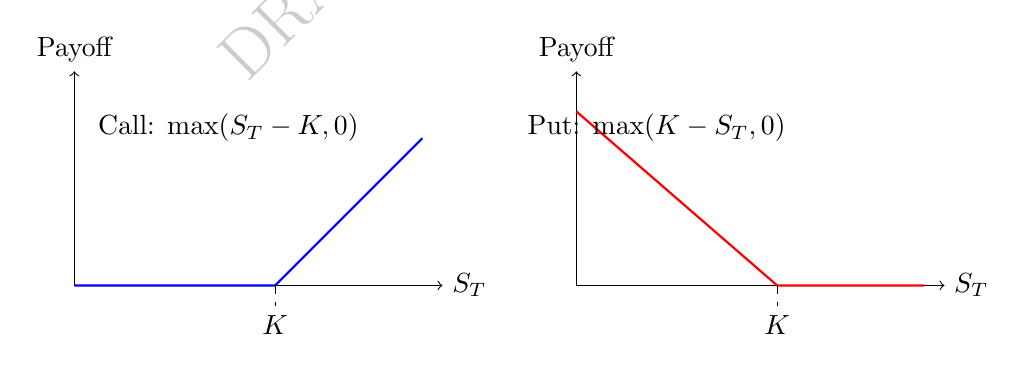
\begin{tikzpicture}[scale=0.85]
        \begin{scope}
            \draw[->] (0,0) -- (5.5,0) node[right] {$S_T$};
            \draw[->] (0,0) -- (0,3.2) node[above] {Payoff};
            \draw[thick,blue] (0,0) -- (3,0) -- (5.2,2.2);
            \draw[dashed] (3,0) -- (3,-0.3) node[below] {$K$};
            \node[above] at (2.3,2.0) {Call: $\max(S_T-K,0)$};
        \end{scope}
        \begin{scope}[xshift=7.5cm]
            \draw[->] (0,0) -- (5.5,0) node[right] {$S_T$};
            \draw[->] (0,0) -- (0,3.2) node[above] {Payoff};
            \draw[thick,red] (0,2.6) -- (3,0) -- (5.2,0);
            \draw[dashed] (3,0) -- (3,-0.3) node[below] {$K$};
            \node[above] at (1.2,2.0) {Put: $\max(K-S_T,0)$};
        \end{scope}
    \end{tikzpicture}
    \caption{Payoff at maturity for a call option (left) and a put option (right) with strike $K$. Both payoffs are piecewise linear and nonnegative, but neither is a linear function of $S_T$ over its full range, which is why options require a replication or no-arbitrage argument to price rather than simple discounting.}
    \label{fig:option_payoffs}
\end{figure}

Because these payoffs are nonlinear functions of the future price, options cannot be priced by simple discounting; instead, they are priced by constructing a replicating portfolio of the underlying asset and a risk-free bond that produces the same payoff in every future state, and then invoking the no-arbitrage principle introduced in Chapter 3: two portfolios with identical payoffs must have the same price today.

The simplest version of this argument is the one-step binomial model\index{binomial option pricing model}. Suppose a stock currently trades at $S_0 = \$50$ and, over one period, either rises to $S_0 u$ or falls to $S_0 d$, with $u=1.2$ and $d=0.9$. A risk-free investment over the same period grows by a gross factor $R = 1+r_f = 1.04$. Consider a call option struck at $K=\$50$. The stock will be worth $S_u = 60$ or $S_d = 45$, so the call will be worth $C_u = \max(60-50,0) = \$10$ or $C_d = \max(45-50,0) = \$0$. No-arbitrage pricing gives the option's value today as a discounted expectation under the risk-neutral probability
\begin{equation*}
q = \frac{R-d}{u-d} = \frac{1.04-0.9}{1.2-0.9} = 0.467,
\end{equation*}
so that
\begin{equation*}
C_0 = \frac{1}{R}[q\,C_u + (1-q)\,C_d] = \frac{1}{1.04}[0.467(10) + 0.533(0)] \approx \$4.49.
\end{equation*}
Crucially, $q$ is not the investor's real-world belief about the probability of an up-move; it is the probability implied by the no-arbitrage condition, which is why this is called risk-neutral pricing\index{Risk-Neutral Pricing}. The same logic extends, by adding more steps and shrinking the time interval, to the continuous-time model presented next.

\subsection{Extending to Two Steps}\index{Extending to Two Steps}

A single step is enough to introduce the mechanics, but a multi-step tree is what actually converges to the Black-Scholes-Merton\index{Black-Scholes-Merton Model} price, as the companion notebook demonstrates numerically for tree sizes up to 5,000 steps. Extending the same stock and option to two periods, each still with $u=1.2$, $d=0.9$, $R=1.04$, produces three possible terminal prices: $S_{uu} = 50(1.2)^2 = \$72$, $S_{ud} = 50(1.2)(0.9) = \$54$, and $S_{dd} = 50(0.9)^2 = \$40.50$, with call payoffs $C_{uu} = \$22$, $C_{ud} = \$4$, and $C_{dd} = \$0$. The risk-neutral probability $q=0.467$ is unchanged, since it depends only on $u$, $d$, and $R$, not on the number of steps, so the tree is solved by working backward one period at a time:
\begin{equation*}
C_u = \frac{1}{R}[q\,C_{uu} + (1-q)\,C_{ud}] = \frac{1}{1.04}[0.467(22) + 0.533(4)] \approx \$11.92, 
\qquad C_d = \frac{1}{R}[q\,C_{ud} + (1-q)\,C_{dd}] \approx \$1.79,
\end{equation*}
\begin{equation*}
C_0 = \frac{1}{R}[q\,C_u + (1-q)\,C_d] \approx \$6.27.
\end{equation*}
This two-step price of \$6.27 is already closer to the Black-Scholes-Merton price of \$6.88 computed later in this chapter than the one-step price of \$4.49 was, consistent with the convergence pattern shown numerically in the companion notebook: as the number of steps grows and each step covers a shorter interval, the binomial price converges to the continuous-time Black-Scholes-Merton price.

The $u=1.2$ and $d=0.9$ used above were chosen for hand-computability, not to represent a specific step size; a tree with an arbitrary number of steps instead derives $u$ and $d$ from the underlying's annualized volatility using the Cox-Ross-Rubinstein\index{Cox-Ross-Rubinstein (CRR) parametrization} parametrization $u=e^{\sigma\sqrt{\Delta t}}$, $d=1/u$, where $\Delta t$ is the length of one step, so that every tree, regardless of how many steps it has, reflects the same annualized volatility $\sigma$. Table~\ref{tab:binomial_convergence} prices the same at-the-money call ($S_0=K=\$50$, $r=4\%$, $\sigma=30\%$, $T=1$ year) with a CRR tree of increasing step count; the price oscillates while converging, but the error shrinks steadily, from \$1.40 at one step to under \$0.001 by 5,000 steps, confirming that the Black-Scholes-Merton formula is exactly the limit this discrete tree approaches as the step size shrinks toward zero.

\begin{table}[htbp]
\centering
\caption{Convergence of the CRR binomial call price to the Black-Scholes-Merton price as the number of steps increases ($S_0=K=\$50$, $r=4\%$, $\sigma=30\%$, $T=1$ year)}
\label{tab:binomial_convergence}
\begin{tabular}{rrr}
\toprule
Steps & Binomial price & Error vs.\ Black-Scholes-Merton \\
\midrule
1     & \$8.28 & +\$1.40 \\
2     & \$6.21 & $-$\$0.67 \\
5     & \$7.16 & +\$0.28 \\
20    & \$6.80 & $-$\$0.07 \\
100   & \$6.86 & $-$\$0.01 \\
500   & \$6.874 & $-$\$0.003 \\
1{,}000 & \$6.875 & $-$\$0.001 \\
5{,}000 & \$6.876 & $-$\$0.0003 \\
\midrule
$\infty$ (Black-Scholes-Merton) & \$6.8766 & --- \\
\bottomrule
\end{tabular}
\end{table}

Figure~\ref{fig:binomial_tree} lays out the full tree, alongside its American put counterpart introduced below, side by side: stock prices grow forward from $S_0$ on the left to three recombining terminal nodes on the right, while option values are computed in the opposite direction, starting from the known terminal payoffs and working backward one period at a time using $q$.

\subsection{American Options and Early Exercise}\index{American Options and Early Exercise}
\label{sec:american-options}

Every option considered so far has been European, exercisable only at maturity. An American option can be exercised at any time up to and including maturity, and the binomial tree extends naturally to price this feature: at each node, compare the value of exercising immediately (the intrinsic value) to the value of continuing to hold the option, and take whichever is larger.

Consider an American put with the same two-period tree and strike $K=\$50$. At maturity the payoffs are unchanged: $P_{uu}=\$0$, $P_{ud}=\$0$, $P_{dd}=\max(50-40.50,0)=\$9.50$. Working backward, the European continuation value at the down node ($S_d=\$45$ after one down move) is $P_d^{\text{cont}} = [q(0) + (1-q)(9.50)]/1.04 \approx \$4.87$. But immediate exercise at that node is worth $\max(50-45,0)=\$5.00$, which exceeds the continuation value, so an optimal holder would exercise early rather than wait: $P_d^{\text{American}} = \max(5.00, 4.87) = \$5.00$. At the up node, both exercise and continuation are worth \$0 (the put is out of the money after an up move), so $P_u^{\text{American}}=\$0$. Rolling back to today, the continuation value is $[q(0) + (1-q)(5.00)]/1.04 \approx \$2.56$, and since immediate exercise today is worth $\max(50-50,0)=\$0$, the American put is worth $P_0^{\text{American}} \approx \$2.56$.

By contrast, the European put (never allowed to exercise early) is worth only $P_0^{\text{European}} \approx \$2.50$, computed by discounting the same terminal payoffs without ever checking intrinsic value along the way. The American put's extra \$0.07 of value (the two full-precision values are \$2.5641 and \$2.4984; the gap only looks like \$0.06 if the two prices are first rounded to the nearest cent and then subtracted) is called the early-exercise premium, and it exists specifically because it was optimal to exercise early at the down node. This early-exercise feature is the reason American puts (and, when the underlying pays dividends, American calls) generally cannot be priced with a simple closed-form formula like Black-Scholes-Merton and instead require a tree, a finite-difference method, or a simulation-based approach that can check the exercise decision at every point in time.

Figure~\ref{fig:binomial_tree} places both trees side by side for direct comparison. The two share identical stock prices throughout, since $u$, $d$, and $q$ never depended on which option is being priced; only the option values in the bottom line of each node differ. The asterisk at the American put's down node marks exactly where the two trees' logic diverges: every other node's value is a plain discounted expectation of its children, but $P_d=\$5.00$ replaces what would otherwise be a \$4.87 continuation value, because immediate exercise is worth more there. That single substitution is the entire early-exercise premium, and it is also why the American put's tree cannot be collapsed into a closed-form formula the way the European call's can.

\begin{figure}[htbp]
    \centering
    \begin{minipage}{0.48\linewidth}
        \centering
        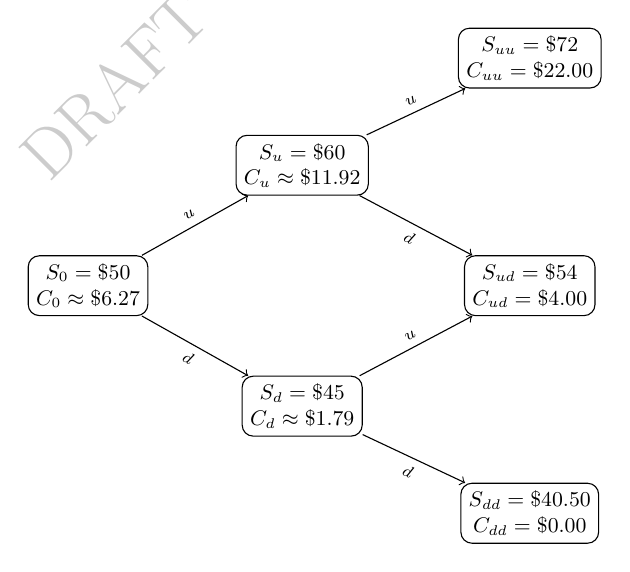
\begin{tikzpicture}[scale=0.85,transform shape,every node/.style={font=\small}]
            \node[draw,rounded corners,align=center] (s0) at (0,0) {$S_0=\$50$\\$C_0\approx\$6.27$};
            \node[draw,rounded corners,align=center] (su) at (3.2,1.8) {$S_u=\$60$\\$C_u\approx\$11.92$};
            \node[draw,rounded corners,align=center] (sd) at (3.2,-1.8) {$S_d=\$45$\\$C_d\approx\$1.79$};
            \node[draw,rounded corners,align=center] (suu) at (6.6,3.4) {$S_{uu}=\$72$\\$C_{uu}=\$22.00$};
            \node[draw,rounded corners,align=center] (sud) at (6.6,0) {$S_{ud}=\$54$\\$C_{ud}=\$4.00$};
            \node[draw,rounded corners,align=center] (sdd) at (6.6,-3.4) {$S_{dd}=\$40.50$\\$C_{dd}=\$0.00$};
            \draw[->] (s0) -- node[above,sloped,font=\scriptsize] {$u$} (su);
            \draw[->] (s0) -- node[below,sloped,font=\scriptsize] {$d$} (sd);
            \draw[->] (su) -- node[above,sloped,font=\scriptsize] {$u$} (suu);
            \draw[->] (su) -- node[below,sloped,font=\scriptsize] {$d$} (sud);
            \draw[->] (sd) -- node[above,sloped,font=\scriptsize] {$u$} (sud);
            \draw[->] (sd) -- node[below,sloped,font=\scriptsize] {$d$} (sdd);
        \end{tikzpicture}

        \small European call
    \end{minipage}%
    \hfill
    \begin{minipage}{0.48\linewidth}
        \centering
        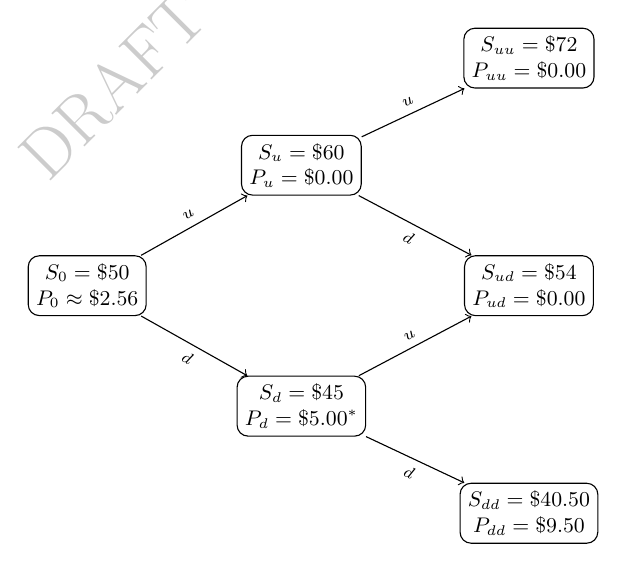
\begin{tikzpicture}[scale=0.85,transform shape,every node/.style={font=\small}]
            \node[draw,rounded corners,align=center] (s0) at (0,0) {$S_0=\$50$\\$P_0\approx\$2.56$};
            \node[draw,rounded corners,align=center] (su) at (3.2,1.8) {$S_u=\$60$\\$P_u=\$0.00$};
            \node[draw,rounded corners,align=center] (sd) at (3.2,-1.8) {$S_d=\$45$\\$P_d=\$5.00^*$};
            \node[draw,rounded corners,align=center] (suu) at (6.6,3.4) {$S_{uu}=\$72$\\$P_{uu}=\$0.00$};
            \node[draw,rounded corners,align=center] (sud) at (6.6,0) {$S_{ud}=\$54$\\$P_{ud}=\$0.00$};
            \node[draw,rounded corners,align=center] (sdd) at (6.6,-3.4) {$S_{dd}=\$40.50$\\$P_{dd}=\$9.50$};
            \draw[->] (s0) -- node[above,sloped,font=\scriptsize] {$u$} (su);
            \draw[->] (s0) -- node[below,sloped,font=\scriptsize] {$d$} (sd);
            \draw[->] (su) -- node[above,sloped,font=\scriptsize] {$u$} (suu);
            \draw[->] (su) -- node[below,sloped,font=\scriptsize] {$d$} (sud);
            \draw[->] (sd) -- node[above,sloped,font=\scriptsize] {$u$} (sud);
            \draw[->] (sd) -- node[below,sloped,font=\scriptsize] {$d$} (sdd);
        \end{tikzpicture}

        \small American put
    \end{minipage}
    \caption{The two-step binomial tree for the \$50-strike European call (left) and American put (right). Both share the same stock-price tree, growing forward from $S_0$ under up- and down-moves $u=1.2$ and $d=0.9$ and recombining at the middle terminal node. Option values (bottom line of each node) are computed backward from the known terminal payoffs using the risk-neutral probability $q=0.467$, except at the American put's down node, marked with an asterisk, where the \$5.00 intrinsic value of immediate exercise replaces the lower \$4.87 continuation value, producing the early-exercise premium discussed in the text.}
    \label{fig:binomial_tree}
\end{figure}

\section{The Black-Scholes-Merton Model}\index{Black-Scholes-Merton Model}

The Black-Scholes-Merton model is the continuous-time limit of the binomial approach and remains the benchmark option pricing formula in both practice and further theoretical work. For a non-dividend-paying stock with current 
price $S_0$, strike $K$, risk-free rate $r$ (continuously compounded), volatility $\sigma$, and time to maturity $T$ (in years), the price of a European call is
\begin{equation*}
C = S_0 N(d_1) - K e^{-rT} N(d_2), \qquad
d_1 = \frac{\ln(S_0/K) + (r+\sigma^2/2)T}{\sigma\sqrt{T}}, \qquad
d_2 = d_1 - \sigma\sqrt{T},
\end{equation*}
where $N(\cdot)$ is the standard normal cumulative distribution function. Using the same at-the-money strike as the binomial example, $S_0 = K = \$50$, with $r = 4\%$, $\sigma = 30\%$, and $T = 1$ year,
\begin{equation*}
d_1 = \frac{0 + (0.04+0.045)(1)}{0.30} = 0.283, \qquad d_2 = 0.283 - 0.30 = -0.017,
\end{equation*}
and looking up $N(0.283) = 0.6115$ and $N(-0.017) = 0.4934$ gives
\begin{equation*}
C = 50(0.6115) - 50\,e^{-0.04}(0.4934) \approx \$6.88.
\end{equation*}
This is noticeably higher than the one-step binomial price of \$4.49 for the same strike and initial price, because the binomial example allowed only two possible outcomes over the full year, 
while Black-Scholes-Merton assumes prices can move continuously and allows for a full year of compounded volatility; a multi-step binomial tree with enough steps converges to the Black-Scholes-Merton price as the step size shrinks. 
The corresponding put price is
\begin{equation*}
P = K e^{-rT} N(-d_2) - S_0 N(-d_1) \approx \$4.92,
\end{equation*}
and the two prices must satisfy put-call parity,
\begin{equation*}
C + K e^{-rT} = P + S_0,
\end{equation*}
which can be checked directly: $6.88 + 50\,e^{-0.04} = 6.88 + 48.04 = \$54.92$, and $4.92 + 50 = \$54.92$, confirming consistency. Put-call parity\index{Put-Call Parity} holds regardless of any particular pricing model, since it follows from no-arbitrage alone; 
it is therefore a useful sanity check on any option pricing implementation, including a machine learning model trained to approximate option prices.

The quantity $N(d_1) = 0.6115$ in this example is also the option's delta, the sensitivity of the option price to a one-dollar change in the stock price, and is the first of several ``Greeks'' used to 
measure and hedge an option position's risk exposures.

\section{The Greeks: Measuring an Option's Risk Exposures}\index{Greeks: Measuring an Option's Risk Exposures}

A market maker who has just sold the call option priced above is exposed to several distinct sources of risk, and each of the Greeks quantifies one of them. Four of the five Greeks below share a single building block: $\phi(\cdot)$, the standard normal probability density function,
\begin{equation*}
\phi(x) = \frac{1}{\sqrt{2\pi}}\,e^{-x^2/2},
\end{equation*}
the height of the standard normal bell curve at $x$, distinct from $N(x)$, the cumulative area under that curve already used to price the option itself. Evaluated at the same $d_1$ computed above, but at full precision ($d_1 = 0.28333$, not the rounded $0.283$ displayed there, since rounding before this step would cascade into every Greek that uses it),
\begin{equation*}
\phi(d_1) = \frac{1}{\sqrt{2\pi}}\,e^{-0.28333^2/2} \approx 0.3832.
\end{equation*}
For a European call under Black-Scholes-Merton,
\begin{align*}
\Delta &= N(d_1), &\text{(sensitivity to the stock price)} \\
\Gamma &= \frac{\phi(d_1)}{S_0 \sigma \sqrt{T}}, &\text{(sensitivity of delta itself to the stock price)} \\
\text{Vega} &= S_0 \phi(d_1) \sqrt{T}, &\text{(sensitivity to volatility)} \\
\Theta &= -\frac{S_0 \phi(d_1) \sigma}{2\sqrt{T}} - r K e^{-rT} N(d_2), &\text{(sensitivity to the passage of time)} \\
\rho &= K T e^{-rT} N(d_2). &\text{(sensitivity to the interest rate)}
\end{align*}
Evaluating each at the same inputs as before ($S_0=K=\$50$, $r=4\%$, $\sigma=30\%$, $T=1$) gives $\Delta = 0.6115$ (already computed), $\Gamma = \phi(d_1)/(50 \times 0.30 \times 1) \approx 0.0255$, $\text{Vega} = 50 \times \phi(d_1) \times 1 \approx 19.16$, $\Theta \approx -3.82$ per year (about $-\$0.0105$ per calendar day), and $\rho = 23.70$ (per unit, i.e., per 100 percentage points, change in the interest rate). The shared $\phi(d_1) \approx 0.3832$ term is exactly why gamma, vega, and theta rise and fall together: whatever pushes $d_1$ closer to zero, the peak of the bell curve, an at-the-money option, or higher volatility relative to how far the stock sits from the strike, simultaneously raises gamma, vega, and the magnitude of theta, while delta and rho depend only on the cumulative-probability terms $N(d_1)$ and $N(d_2)$ and do not share this common driver.

These numbers have direct trading interpretations. Delta of 0.6115 means the option's price moves about \$0.61 for every \$1 move in the stock, which is why a market maker who sold this call would typically hedge by buying 0.6115 shares per option sold, a strategy called delta hedging\index{Delta Hedging}. Gamma of 0.0255 measures how quickly that hedge ratio itself changes as the stock moves, so a market maker must rebalance the hedge more frequently when gamma is high. Vega of 19.16 (often quoted per one percentage point of volatility, so $19.16/100 \approx \$0.19$) shows the option loses or gains meaningful value purely from changes in the market's volatility expectations, entirely independent of the stock price itself, which is exactly the channel through which the volatility clustering discussed in Chapter 7 affects option values. Theta of $-\$3.82$ per year reflects time decay: holding everything else fixed, the option loses value simply as it approaches expiration, since less time remains for the stock to move in the holder's favor.

\subsection*{A Worked Example: Delta Hedging and Its Limits}

Suppose a market maker sells $1{,}000$ of these call options and immediately delta-hedges by buying $1{,}000 \times 0.6115 = 611.5$ shares, funded however the market maker chooses. If the stock rises by \$1, from \$50 to \$51, the hedge's stock position gains $611.5 \times \$1 = \$611.50$. Recomputing the exact Black-Scholes-Merton price at $S=\$51$ (holding every other input fixed) gives a new call price of $\$7.5008$, up from $\$6.8766$, so the short option position loses $1{,}000 \times (7.5008 - 6.8766) = \$624.15$. The hedge does not offset this loss exactly: the net result is a loss of $611.50 - 624.15 = -\$12.65$, small relative to the \$1,000-contract position but not zero, purely because delta is only a first-order (linear) approximation of how the option's price actually responds to the stock price, exactly the same limitation this chapter's modified-duration approximation for a bond's price-yield relationship has.

Just as convexity corrected the bond-duration approximation, gamma corrects the delta approximation here: the delta-only prediction for the new option price is $C_0 + \Delta(S_1-S_0) = 6.8766 + 0.6115(1) = \$7.4882$, while adding the gamma correction, $C_0 + \Delta(S_1-S_0) + \tfrac{1}{2}\Gamma(S_1-S_0)^2 = 7.4882 + 0.5(0.0255)(1)^2 \approx \$7.5009$, lands almost exactly on the true recomputed price of \$7.5008. A market maker who rebalances a delta hedge only occasionally, rather than continuously, is therefore always exposed to some residual gamma risk between rebalances, larger for bigger stock moves (since the gamma correction term grows with the square of the price change) and larger for options with higher gamma, exactly the at-the-money, short-time-to-expiration options this section already flagged as having the largest gamma. This is precisely why professional options market makers monitor and actively manage gamma, not just delta, and why a large, sudden price move is disproportionately costly to a delta-hedged options book relative to a series of small moves of the same total size.

\section{Implied Volatility}\index{Implied Volatility}

The Black-Scholes-Merton formula takes $\sigma$ as an input and produces a price as output. In practice, market participants often run this relationship in reverse: given an observed market price for an option, they solve for the volatility that the Black-Scholes-Merton formula would need in order to reproduce that price, called the implied volatility. Because the formula is not easily invertible algebraically, implied volatility is typically found numerically, using the same kind of root-finding procedure introduced for bond yield to maturity in Section 5.3.

Suppose the same call option (the one priced at \$6.88 under an assumed volatility of 30\%) is instead observed trading in the market at \$7.50. 
The implied volatility $\hat\sigma$ solves $C_{BS}(\hat\sigma) = 7.50$, which a numerical solver finds to be $\hat\sigma \approx 33.25\%$, noticeably 
higher than the 30\% originally assumed. This gap is informative: it means the market is pricing in more uncertainty about the stock's future price 
than the 30\% historical-volatility assumption used earlier in this chapter would suggest, whether because of an upcoming earnings announcement, 
macroeconomic uncertainty, or simply a different market view. Because implied volatility is forward-looking, reflecting the market's current 
expectation rather than a backward-looking historical average, it is often treated as a more useful volatility estimate for pricing other, 
related options than historical volatility is.

If the Black-Scholes-Merton model's constant-volatility assumption held exactly, every option on the same underlying and the same maturity, 
regardless of strike, would imply the same $\hat\sigma$: a call at $K=\$40$ and a call at $K=\$60$ would both back out the same number, because 
the model treats $\sigma$ as a property of the underlying stock, not of the individual option contract. In practice this is not what happens. 
Plotting implied volatility against strike, for options on the same underlying and the same maturity, typically produces a curve, not a flat line, 
and market practitioners distinguish two common shapes. A \textbf{volatility smile}\index{Volatility smile} is roughly symmetric: implied volatility is 
lowest for at-the-money options and rises for both deep in-the-money and deep out-of-the-money strikes, a pattern most associated with currency options, 
where a large move in either direction, a currency crisis or a currency surge, is plausible. A \textbf{volatility skew}\index{Volatility skew}, the 
shape actually observed for equity and equity-index options, is instead mostly downward sloping: implied volatility is highest for low strikes 
(deep in-the-money calls, equivalently far out-of-the-money puts) and falls as the strike rises, so out-of-the-money puts are systematically 
priced as if the stock were more volatile than an at-the-money or out-of-the-money call would suggest. 

Two economic explanations are usually 
offered for the equity skew specifically, and both remain active areas of empirical research rather than settled fact: the \emph{leverage effect} (Black, 1976), whereby a falling stock price mechanically raises a levered firm's debt-to-equity ratio and therefore its equity volatility, so low-strike, low-stock-price states are genuinely more volatile ones; and \emph{crash risk}, sometimes called ``crashophobia'' (Rubinstein, 1994), the observation that the pronounced equity skew now taken for granted was far less visible in listed U.S. index option prices before the October 1987 crash, and that persistent demand for downside protection, buying out-of-the-money puts as portfolio insurance, has kept those puts priced at a premium (equivalently, a higher implied volatility) ever since.

\subsection*{A Worked Example: Computing an Implied Volatility Skew}

The single implied-volatility computation above generalizes directly: solving $C_{BS}(\hat\sigma) = \text{market price}$ separately at each strike, holding $S_0=\$50$, $r=4\%$, and $T=1$ year fixed throughout, traces out the skew itself rather than only describing it in the abstract. Table~\ref{tab:vol_skew} does exactly this for five hypothetical market prices spanning strikes of \$40 to \$60, including the \$50 at-the-money option already solved above.

\begin{table}[htbp]
\centering
\caption{Implied volatilities solved from five one-year call option market prices on the same underlying ($S_0=\$50$, $r=4\%$)}
\label{tab:vol_skew}
\begin{tabular}{cccc}
\toprule
Strike ($K$) & Market price & $d$ (moneyness, $S_0-K$) & Implied volatility \\
\midrule
\$40 & \$14.23 & $+\$10$ (in-the-money)      & 40.02\% \\
\$45 & \$10.57 & $+\$5$                        & 36.00\% \\
\$50 & \$7.50  & \$0 (at-the-money)            & 33.25\% \\
\$55 & \$4.20  & $-\$5$                        & 26.92\% \\
\$60 & \$2.19  & $-\$10$ (out-of-the-money)    & 24.00\% \\
\bottomrule
\end{tabular}
\end{table}

The pattern in Table~\ref{tab:vol_skew} is exactly the equity skew described above, not a symmetric smile: implied volatility falls by roughly 16 percentage points, from 40.02\% down to 24.00\%, as the strike rises from \$40 to \$60, with the single largest drop, more than six points, occurring between the \$50 and \$55 strikes. A trader reading this table would conclude that the market is pricing meaningfully more downside risk into this stock than a single, constant-volatility Black-Scholes-Merton price would imply: the far-out-of-the-money \$60 call is priced as if volatility were only 24\%, while the deep-in-the-money \$40 call, equivalent by put-call parity to a far-out-of-the-money put, is priced as if volatility were 40\%, sixteen points higher.

Table~\ref{tab:vol_skew} fixes maturity at one year and varies only the strike, a single one-dimensional slice through what is, in general, a genuinely two-dimensional object. Repeating the same exercise with $T=0.25$ (three months) instead of one year, holding $S_0$, $r$, and the same five strikes fixed, produces a second slice:
\begin{align*}
K=\$40: &\ 47.03\%, & K=\$45: &\ 40.04\%, & K=\$50: &\ 33.55\%, \\
K=\$55: &\ 27.04\%, & K=\$60: &\ 24.48\%. & &
\end{align*}
Figure~\ref{fig:vol_skew} plots both slices together. Two things stand out. First, both curves slope downward, confirming the skew shape is not specific to a single maturity. Second, and more informative, the two curves are not simply parallel: the three-month curve sits noticeably above the one-year curve at low strikes ($47.03\%$ versus $40.02\%$ at $K=\$40$, a gap of nearly seven points) but the two curves nearly converge at high strikes ($24.48\%$ versus $24.00\%$ at $K=\$60$, under half a point apart). The three-month skew is therefore steeper than the one-year skew, a well-documented empirical pattern: near-term crash protection is priced at a particularly large premium, since a crash is by definition a short, sudden event, while longer-dated options have more time for volatility to mean-revert toward its long-run average, flattening the skew somewhat. This joint variation across both strike and maturity, not strike alone, is precisely what the \textbf{volatility surface}\index{Volatility surface} refers to: a full grid of implied volatilities, one for every combination of strike and maturity actively traded, of which Table~\ref{tab:vol_skew} and its three-month counterpart are two single-maturity cross-sections.

\begin{figure}[htbp]
    \centering
    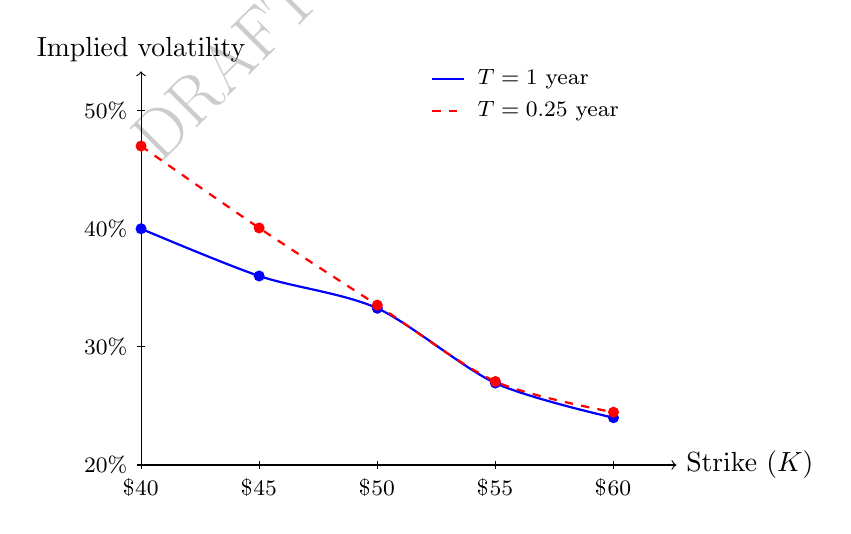
\begin{tikzpicture}[scale=1.0]
        \draw[->] (0,0) -- (6.8,0) node[right] {Strike ($K$)};
        \draw[->] (0,0) -- (0,5.0) node[above] {Implied volatility};
        \foreach \x/\lbl in {0/\$40, 1.5/\$45, 3/\$50, 4.5/\$55, 6/\$60} {
            \draw (\x,0.05) -- (\x,-0.05) node[below,font=\footnotesize] {\lbl};
        }
        \foreach \y/\lbl in {0/20\%, 1.5/30\%, 3/40\%, 4.5/50\%} {
            \draw (0.05,\y) -- (-0.05,\y) node[left,font=\footnotesize] {\lbl};
        }
        \draw[blue,thick,smooth] plot coordinates {(0,3.00) (1.5,2.40) (3,1.99) (4.5,1.04) (6,0.60)};
        \draw[red,thick,dashed,smooth] plot coordinates {(0,4.05) (1.5,3.01) (3,2.03) (4.5,1.06) (6,0.67)};
        \fill[blue] (0,3.00) circle (2pt);
        \fill[blue] (1.5,2.40) circle (2pt);
        \fill[blue] (3,1.99) circle (2pt);
        \fill[blue] (4.5,1.04) circle (2pt);
        \fill[blue] (6,0.60) circle (2pt);
        \fill[red] (0,4.05) circle (2pt);
        \fill[red] (1.5,3.01) circle (2pt);
        \fill[red] (3,2.03) circle (2pt);
        \fill[red] (4.5,1.06) circle (2pt);
        \fill[red] (6,0.67) circle (2pt);
        \draw[blue,thick] (3.7,4.9) -- (4.1,4.9);
        \node[right,font=\footnotesize] at (4.15,4.9) {$T=1$ year};
        \draw[red,thick,dashed] (3.7,4.5) -- (4.1,4.5);
        \node[right,font=\footnotesize] at (4.15,4.5) {$T=0.25$ year};
    \end{tikzpicture}
    \caption{The implied volatility skew for one-year (solid) and three-month (dashed) call options on the same underlying ($S_0=\$50$, $r=4\%$), from Table~\ref{tab:vol_skew} and its three-month counterpart. Both curves slope downward, the equity skew rather than a symmetric smile, but the three-month curve is visibly steeper, converging with the one-year curve at high strikes while sitting well above it at low strikes.}
    \label{fig:vol_skew}
\end{figure}

\subsection*{Why the Volatility Smile Matters for AI and Machine Learning}

The skew and surface just computed are not just a curiosity for option traders; they are one of the most important places where modern finance meets machine learning. A simple Black-Scholes-Merton model assigns one volatility to every option on the same underlying, but the market does not behave that way, as Table~\ref{tab:vol_skew} and Figure~\ref{fig:vol_skew} showed directly. Options with different strikes and maturities imply systematically different volatilities, differences structured enough to form a rich pattern that can be learned from data. That is why researchers and practitioners use machine learning to model implied-volatility surfaces, to estimate the residual error between theoretical prices and observed market prices, and to build fast pricing or hedging tools for large option books.

The opportunity is attractive because the data are high-dimensional and highly structured: strike, maturity, underlying price, interest rates, and recent market regimes all matter. A machine learning model can learn which combinations of these features predict unusually high or low implied volatility, but it must still respect economic constraints. In particular, the fitted surface should remain economically sensible, avoid producing arbitrage opportunities, and be stable out of sample rather than simply memorizing recent market moves. For that reason, AI and machine learning are best viewed here as tools for capturing patterns in the volatility surface, not as replacements for the no-arbitrage logic that makes option pricing coherent in the first place.

A single option's implied volatility is a useful estimate for that specific contract, but it can be distorted by idiosyncratic events affecting one company, and no single option fully summarizes the market's overall volatility expectations. The CBOE Volatility Index\index{CBOE Volatility Index (VIX)} (VIX), often called the market's ``fear gauge,'' addresses this by aggregating implied volatilities across a wide range of strikes and maturities for S\&P 500 index options into a single number, using a model-free methodology (following Britten-Jones and Neuberger, 2000) that does not require inverting the Black-Scholes-Merton formula for any single option at all, exactly the volatility-surface aggregation the previous paragraph described, now condensed into one tradable index. VIX is quoted as an annualized percentage representing the market's expectation of S\&P 500 volatility over the next 30 days; it typically trades in the neighborhood of $12\%$ to $20\%$ during calm markets and spiked above $80\%$ during the most acute phases of both the 2008 financial crisis and the March 2020 COVID-19 selloff, a graphic illustration of how quickly the market's own volatility expectations can move relative to the historical-volatility assumptions used earlier in this chapter. Because VIX is itself directly tradable, through VIX futures, options, and exchange-traded products, it recurs later in this book as a market-wide risk signal distinct from any single asset's own volatility: Chapter 11 uses it as a regime filter for trading strategies, and Chapter 14 treats it as a price-based complement to text-based sentiment measures.

Figure~\ref{fig:ch5-vix} shows VIX's actual daily closing history from its 1990 inception through the most recent available date, downloaded directly from Yahoo Finance, with several of its largest spikes labeled: the 1998 collapse of Long-Term Capital Management amid the Russian sovereign default (examined in detail in Chapter 3), the September 2001 terrorist attacks, the mid-2002 selloff accompanying the WorldCom bankruptcy and the broader wave of corporate accounting scandals that closed out the dot-com bear market, the 2008 global financial crisis, the May 2010 Flash Crash (Chapter 3's own case study), the August 2011 U.S. sovereign credit rating downgrade, the August 2015 selloff triggered by a surprise Chinese currency devaluation and fears of a slowing Chinese economy, the February 2018 ``Volmageddon'' collapse of short-volatility exchange-traded products, the March 2020 COVID-19 selloff, the August 2024 yen carry-trade unwind, when a surprise Bank of Japan rate hike collided with a weak U.S. jobs report and briefly sent VIX to an intraday high of $65.73$ before it closed the session at $38.57$, and the April 2025 tariff war, when a sweeping new round of U.S. tariff announcements drove VIX to a closing high of $52.33$, its third-highest close on record behind only 2008 and 2020. Every spike shares the same shape: VIX otherwise drifts in a comparatively narrow band, roughly $10\%$ to $20\%$, then jumps sharply to $40\%$-$80\%$ or more within days whenever a shock forces the market to reprice risk abruptly, before subsiding again once the acute phase of the shock passes, exactly the kind of volatility clustering and mean reversion modeled directly in Chapter 7's GARCH(1,1) recursion. Not every geopolitical shock produces a comparable spike: the June 2025 Israel-Iran conflict and the accompanying U.S. strikes on Iranian nuclear facilities, for instance, left VIX only modestly elevated, in the low twenties, a reminder that VIX reprices the market's expectation of \emph{equity} volatility specifically, and a shock has to threaten broad equity cash flows or risk appetite, not merely be geopolitically significant, to move it sharply.

\begin{figure}[htbp]
    \centering
    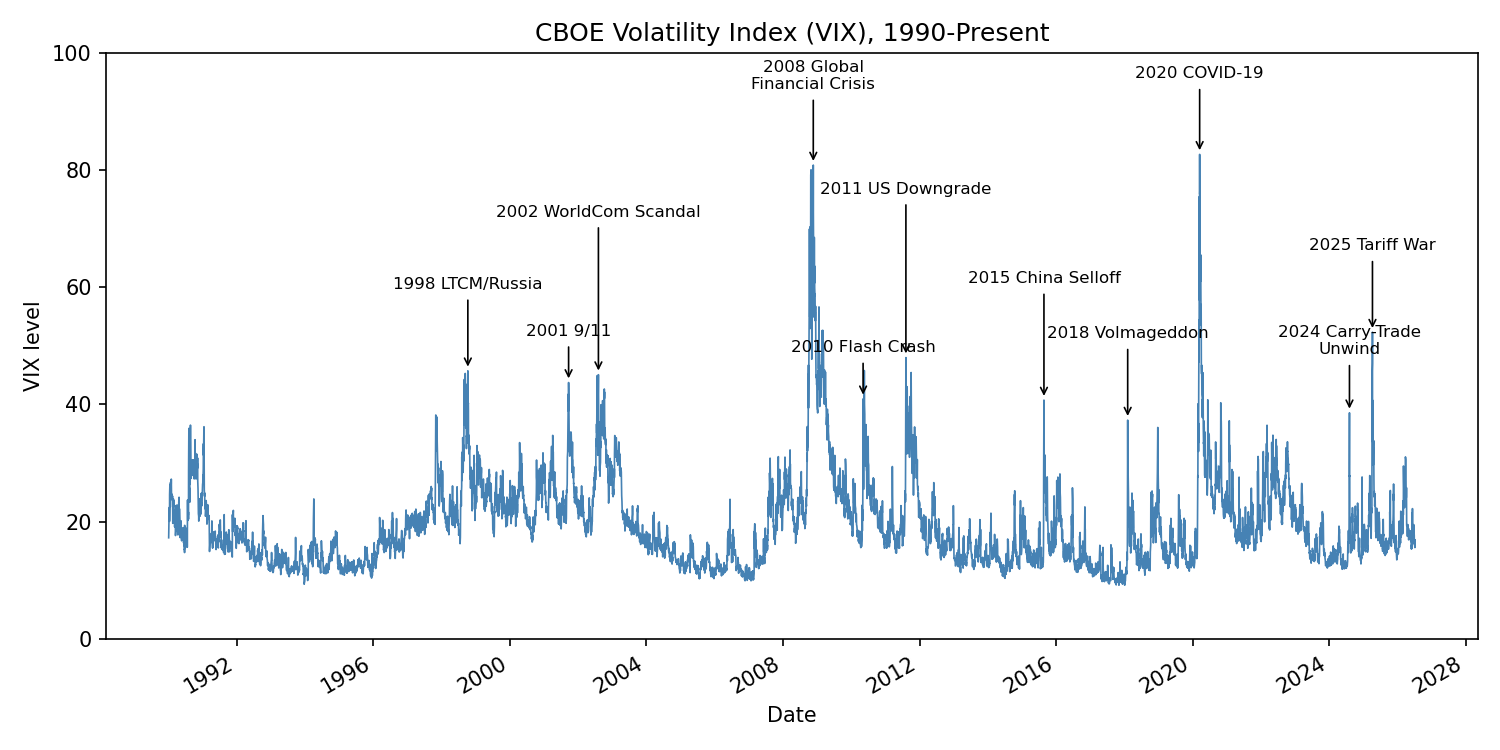
\includegraphics[width=\linewidth]{ch5_fig_vix.png}
    \caption{The CBOE Volatility Index (VIX), daily closes from January 1990 through the most recent available date, downloaded via the \texttt{yfinance} library. Labeled spikes mark, from left to right, the 1998 LTCM/Russia crisis (VIX $45.74$), the September 2001 terrorist attacks (VIX $43.74$), the 2002 WorldCom accounting-scandal selloff (VIX $45.08$), the 2008 global financial crisis (VIX $80.86$), the May 2010 Flash Crash (VIX $40.95$), the August 2011 U.S. credit rating downgrade (VIX $48.00$), the August 2015 China selloff (VIX $40.74$), the February 2018 Volmageddon episode (VIX $37.32$), the March 2020 COVID-19 selloff, VIX's all-time closing high of $82.69$, the August 2024 yen carry-trade unwind (VIX closed at $38.57$ after an intraday high of $65.73$), and the April 2025 tariff war (VIX $52.33$).}
    \label{fig:ch5-vix}
\end{figure}

\section{Real Options: Applying Option Pricing to Corporate Decisions}\index{Real Options: Applying Option Pricing to Corporate Decisions}

The option pricing machinery developed in this chapter for financial derivatives applies, with some adaptation, to certain corporate investment decisions as well, an application known as real options analysis. The insight is that many corporate decisions have an option-like structure: a firm has the right, but not the obligation, to take some action, and can choose whether and when to exercise that right based on how conditions evolve.

Consider a mining company deciding whether to develop a mineral deposit. A standard net-present-value calculation would estimate a single expected value for the project and approve it only if that value is positive. But the firm actually holds something closer to a call option: it can wait, observe how commodity prices evolve, and develop the deposit only if prices rise enough to make it profitable, walking away (at the cost of whatever it spent on exploration and permitting) if prices fall instead. This option to wait has value, exactly as the extra flexibility embedded in an American option (Section~\ref{sec:american-options}) has value beyond its European counterpart, and a standard net-present-value analysis that ignores this flexibility can systematically undervalue the opportunity.

Other common examples include the option to expand a successful pilot project, the option to abandon a failing project and salvage its assets, and the option to switch between input sources or output products as relative prices change. In each case, the underlying ``asset'' is the value of the future cash flows the decision affects, the ``strike price'' is the cost of taking the action, and volatility in the underlying business or commodity price plays exactly the same role it plays in the Black-Scholes-Merton formula: more uncertainty makes the option to wait, expand, or abandon more valuable, not less, since flexibility is most useful precisely when the future is most uncertain. This is a genuinely counterintuitive result relative to naive intuition (which often treats uncertainty as purely a negative), and it is one of the most important practical lessons real options analysis contributes to corporate finance. Real options are typically harder to value precisely than financial options, since the ``underlying asset'' rarely trades in a liquid market with an observable volatility, but the qualitative logic, that flexibility has value and that value increases with uncertainty, remains a useful lens for evaluating investment decisions even when a precise Black-Scholes-Merton-style number is not available.

A simplified numerical illustration makes the option-to-wait logic concrete, even without a fully specified binomial tree of traded prices. Suppose the mining company's deposit costs $K = \$50$ million to develop, and, if developed today, is worth exactly $\$50$ million, a marginal project with $\text{NPV} = 50.0 - 50.0 = \$0$ that a naive analysis would treat as a coin flip, worth doing but not clearly attractive. Suppose that if the firm waits one year, the deposit's value will have moved to either $\$70$ million (if commodity prices rise) or $\$35$ million (if they fall), each with probability $0.5$, and the firm develops the deposit only if doing so is still profitable at that point. The expected payoff from waiting is
\begin{equation*}
E[\text{Payoff}] = 0.5 \times \max(70.0 - 50.0,\ 0) + 0.5 \times \max(35.0 - 50.0,\ 0) = 0.5(20.0) + 0.5(0) = \$10.0 \text{ million},
\end{equation*}
which, discounted one year at a risk-free rate of $5\%$, has a present value of $10.0/1.05 \approx \$9.52$ million, substantially higher than the $\$0$ NPV of developing immediately. The value of waiting comes entirely from the asymmetry built into the option to walk away: the firm captures the full upside if prices rise but avoids the downside entirely if they fall, an asymmetry a simple point-estimate NPV calculation, which implicitly commits to developing the project regardless of how prices move, cannot capture at all. This is exactly why a corporate finance team that evaluates a marginal project using only a single expected NPV, without asking whether waiting for more information is itself a valuable and available choice, can systematically pass over projects, or approve them prematurely, in ways that ignore real, quantifiable option value.

\section{Putting It Together: Valuing Meridian Fabrication}\index{Putting It Together: Valuing Meridian Fabrication}

This chapter has now developed both major approaches to valuing a business, discounted cash flow and relative valuation multiples, and it is worth applying both to Meridian Fabrication side by side, using the WACC computed earlier in this chapter, to see how differently they can answer the same question.

For the DCF approach, suppose Meridian's free cash flow, currently $-\$8.0$ million in Year 2 (Chapter 4), gradually recovers as its working-capital investment matures: $-\$2.0$ million in Year 3, $\$3.0$ million in Year 4, and $\$6.0$ million in Year 5, after which free cash flow grows at a stable long-run rate of $g=3\%$ forever. Discounting at the full-precision WACC of $7.342\%$ computed earlier in this chapter (before rounding to $7.34\%$ for display),
\begin{equation*}
PV(\text{Years 3-5 FCF}) = \frac{-2.0}{1.07342} + \frac{3.0}{1.07342^2} + \frac{6.0}{1.07342^3} \approx \$5.59 \text{ million},
\end{equation*}
and the terminal value at the end of Year 5, using the Gordon growth formula on Year 6's free cash flow, is
\begin{equation*}
TV_5 = \frac{6.0(1.03)}{0.07342 - 0.03} \approx \$142.33 \text{ million}, \qquad PV(TV_5) = \frac{142.33}{1.07342^5} \approx \$99.87 \text{ million}.
\end{equation*}
The DCF enterprise value is $5.59 + 99.87 \approx \$105.47$ million, and subtracting net debt of $\$58.0 - \$9.0 = \$49.0$ million gives an implied equity value of approximately $\$56.47$ million.

Compare this to the multiples-based equity value computed in Section 5.8: $\$107.0$ million, nearly twice as large. Both are legitimate valuation methods applied to the same company; the large gap between them reflects a real economic disagreement, not a computational error. The DCF value is driven by Meridian's own, currently weak, cash generation and its slow projected recovery, while the multiples value assumes Meridian deserves to trade at the same EBITDA multiple as healthier comparable firms, effectively assuming its cash flow problems are temporary and will not persist. Interestingly, the DCF-implied equity value of \$56.47 million is still fairly close to Meridian's \$54.0 million book value of equity, while the multiples-based value is far above it, which itself is informative: it suggests the DCF assumptions are the more conservative, and arguably the more defensible, starting point until there is concrete evidence, such as an improving cash conversion cycle or margin expansion, that Meridian's operating performance is converging toward that of its healthier peers. This kind of triangulation across methods, and an honest accounting of why they disagree, is standard practice in real valuation work and is a more useful output than any single number produced by either method alone. In practice, the analyst would not stop at the two values; the next step would be to test how much each estimate changes under alternative market multiples, discount rates, and cash-flow scenarios. That sensitivity analysis is often more informative than the point estimate itself.

\section{Challenges in Valuation and Asset Pricing}

The models in this chapter are elegant and, within their assumptions, exact. Applying them to real markets introduces several recurring challenges.

\textbf{Discount-rate uncertainty.} Every model in this chapter takes $r$ as given, but in practice the discount rate itself must be estimated, typically from an asset pricing model such as the CAPM or a multi-factor model (covered in Chapter 10), and estimates of the required return can vary substantially across reasonable methodologies. Since the Gordon growth model shows that price is extremely sensitive to $r-g$, uncertainty in $r$ translates directly into wide uncertainty in fair value.

\textbf{Volatility is not observed, only estimated.} The Black-Scholes-Merton formula requires $\sigma$, the volatility of the underlying asset, but $\sigma$ cannot be observed directly; it must be estimated from historical returns or backed out from other option prices as an ``implied volatility.'' Different estimation windows and methods can produce meaningfully different prices for the same option, and volatility itself changes over time, which is precisely the motivation for the GARCH-family models introduced in Chapter 7.

\textbf{Model risk and the limits of closed-form pricing.} Every closed-form pricing model rests on simplifying assumptions, constant volatility and continuous trading for Black-Scholes-Merton, a flat and unchanging growth rate for the Gordon growth model, no default risk in the basic bond pricing formula. Real markets violate all of these to varying degrees, and a model that is used outside the range of conditions it was built for can silently produce a confidently wrong price, a risk usually called model risk.

\textbf{Credit risk complicates bond pricing.} The bond pricing formula in this chapter assumes the promised cash flows are paid with certainty. A corporate bond carries default risk, so its price reflects both discounting and the probability-weighted possibility of missed payments, which requires the credit models developed in Chapter 9.

\textbf{Calibration\index{calibration} versus estimation at scale.} A trading desk must reprice large portfolios of derivatives continuously as market conditions change, which requires the underlying models to be calibrated quickly and consistently across thousands of instruments. This operational requirement, not just theoretical accuracy, is a major reason simpler closed-form models such as Black-Scholes-Merton remain in wide use even though more elaborate stochastic volatility and jump-diffusion model\index{diffusion model}s are known to fit historical data better.

\textbf{Where machine learning fits in.} Because closed-form models are known to deviate from observed market prices in systematic ways (the volatility smile is a direct symptom), researchers and practitioners have used machine learning both to learn the deviation directly (predicting the gap between a model price and the observed market price) and to learn pricing functions or implied volatility surfaces end to end from data. These approaches can capture patterns a fixed formula cannot, but they inherit the same risk-management burden as any other statistical model, including the overfitting\index{overfitting} and non-stationarity concerns raised in Chapter 6: a pricing model trained on historical option data can fail exactly when market conditions shift away from the training regime, which is usually when accurate pricing matters most.

\textbf{The term structure adds a further layer of estimation risk.} Section 5.5's yield curve discussion showed that a single discount rate is itself a simplification; a full analysis requires an entire curve of spot rates, and that curve must itself be estimated (typically by ``bootstrapping'' it from a set of observed bond prices), which introduces additional model choices and potential errors before any single bond or derivative is even priced.

\textbf{Real options are hard to value precisely.} The real options perspective introduced in Section 5.13 is conceptually powerful but practically difficult to apply with the same precision as a financial option, since the underlying asset (the value of a future business opportunity) rarely has an observable market price or a clean, constant volatility estimate, which means real options analysis is often used qualitatively, to check whether a standard net-present-value calculation is missing significant flexibility value, rather than to produce a single definitive price.

\textbf{Relative valuation inherits the market's own mistakes.} The multiples-based approach in Section 5.8 depends entirely on comparable companies being reasonably priced; if an entire sector is experiencing a speculative bubble or an unwarranted sell-off, a multiples-based valuation will simply reproduce that mispricing for the target firm rather than correct for it, since the method is explicitly designed to price an asset relative to its peers, not relative to a first-principles estimate of intrinsic value. This is precisely why the DCF-versus-multiples comparison in Section 5.14 is best treated as informative even, and perhaps especially, when the two methods disagree substantially.

\textbf{Illiquidity complicates every valuation approach.} All of the methods in this chapter implicitly assume that once a fair value is computed, an investor could transact at or near that value. For a private company, a thinly traded bond, or a large block of stock relative to average trading volume, this assumption can fail badly: the price actually realizable in a sale may differ meaningfully from any of the theoretical values computed in this chapter, simply because there are too few willing counterparties, echoing the liquidity and market-impact themes of Chapter 3.

\section{Key Takeaways}

Every valuation problem in this chapter reduces to the same idea: discount the relevant future cash flows, or replicate the relevant future payoff, at a rate or under a probability measure consistent with no arbitrage. Bond pricing, the dividend discount model, and option pricing look like different subjects, but they are the same present-value logic applied to progressively more complex cash flow structures, from a fixed schedule of coupons, to a growing perpetuity of dividends, to a payoff that depends nonlinearly on another asset's future price. The chapter's worked examples showed both how to compute these prices and where the underlying models are known to break down, since a practitioner who can only compute a textbook price without understanding its assumptions is exposed to exactly the kind of model risk described above.

The chapter also connected valuation directly to the statements and institutions covered earlier in the book. The WACC example in Section 5.6 discounted Meridian Fabrication's own capital structure from Chapter 4, showing exactly how a firm's balance sheet feeds into the rate used to value it. The credit-risk-adjusted bond price in Section 5.3 previewed the probability-of-default and recovery-rate concepts that Chapter 9's credit models estimate statistically rather than assume. And the Greeks and implied volatility material showed that even a formula as elegant as Black-Scholes-Merton is best understood as a lens for organizing risk exposures and market expectations, rather than as a black box that simply outputs a single correct price. Carrying this perspective, elegant models as organizing frameworks, not oracles, forward is exactly the mindset the rest of this book tries to instill.

The closing Meridian valuation in Section 5.14 is perhaps the single most important exercise in the chapter to internalize, precisely because it did not produce a single answer. A DCF value of \$56.47 million and a multiples-based value of \$107.0 million are both defensible, both computed correctly from the formulas in this chapter, and yet they disagree by nearly a factor of two. Two further points follow from this. First, the disagreement itself is informative: it isolates exactly which assumption, Meridian's own projected cash-flow recovery versus the market's willingness to price it like a healthier peer, is driving the difference, which is a far more useful diagnostic than either number alone. Second, this is exactly the situation a machine learning model trained to predict ``fair value'' from historical data would face silently and without comment: absent an explicit decomposition like the one performed here, a model blending signals from both approaches could produce a single confident-looking number while obscuring a genuine, economically meaningful disagreement about which valuation philosophy is more appropriate for this specific company at this specific time. Preserving, rather than collapsing, this kind of interpretability is a theme this book returns to directly in Chapter 16.

\section{Suggested Exercises}

The exercises below draw on every major tool developed in this chapter, bond pricing and duration, the dividend discount model, binomial and Black-Scholes-Merton option pricing, the cost of capital, and relative valuation, and several build directly on the Meridian Fabrication and Solstice Robotics examples carried over from Chapter 4, so that the numbers you compute here can be checked against, and interpreted alongside, that earlier analysis.

\begin{enumerate}
    \item A 2-year bond with face value \$1,000 and an annual coupon rate of 6\% is priced at a market yield of 8\%. Compute its price using the discounting formula from Section 5.3.
    \item Using the Gordon growth model, find the fair price of a stock expected to pay a dividend of \$2.50 next year, assuming a required return of 10\% and a long-run dividend growth rate of 6\%. Then recompute the price assuming growth of 8\% instead, and comment on how sensitive the price is to this one-percentage-point change.
    \item Using the one-step binomial model with $S_0 = \$40$, $u = 1.25$, $d = 0.8$, $R = 1.05$, and strike $K = \$40$, compute the risk-neutral probability $q$ and the fair price of a call option today.
    \item Verify put-call parity using the Black-Scholes-Merton call and put prices computed in Section 5.10, and explain in your own words why put-call parity must hold regardless of which option pricing model is used.
    \item Using the two-stage dividend discount model from Section 5.7, compute the fair price of a stock with $D_0=\$2.00$, a high-growth rate of $g_1=15\%$ for the first 4 years, a terminal growth rate of $g_2=5\%$, and a required return of $r=11\%$. What fraction of the total price comes from the terminal value?
    \item A 3-year bond with a Macaulay duration of 2.86 years is priced at \$947.51 when $y=7\%$. Use the modified-duration approximation to estimate its price if the yield falls to 6\%, then explain, using the concept of convexity, whether you would expect the approximation to overstate or understate the exact repriced value.
    \item Explain why the Gordon growth model is more sensitive to estimation error than the bond pricing formula in this chapter, referencing the discount-rate uncertainty challenge in Section 5.15.
    \item Describe one concrete way a Black-Scholes-Merton-based pricing system could fail silently (produce a confident but wrong price) if market conditions moved outside the model's assumptions.
    \item Compute Meridian's WACC using Section 5.6's formulas if its equity beta were 0.9 instead of 1.2, holding all other inputs (risk-free rate, market risk premium, cost of debt, tax rate, and capital structure) fixed, and explain the direction of the change.
    \item Using the Greek formulas in Section 5.11, explain why gamma is largest for an option that is close to at-the-money ($S_0 \approx K$) and smaller for options that are deep in- or out-of-the-money, without necessarily recomputing the formula numerically.
    \item A sixth call option on the same stock (still $S_0=\$50$, $r=4\%$, $T=1$), with a strike of $K=\$65$, trades in the market at \$1.00. Using the same numerical root-finding approach used to build Table~\ref{tab:vol_skew}, solve for its implied volatility, and explain whether the result is consistent with the skew pattern already observed across the \$40--\$60 strikes in Section 5.12.
    \item Using the portfolio duration formula in Section 5.4, compute the duration of a bond portfolio holding 30\% in a bond with duration 1.5 years, 50\% in a bond with duration 4.0 years, and 20\% in a bond with duration 8.0 years.
    \item Using Table~\ref{tab:yield_curve}, explain in your own words why a corporate bond's yield should be even higher than the government yield at the same maturity, referencing the credit-risk-adjustment concept from Section 5.3.
    \item Using the multiples method in Section 5.8 and Solstice Robotics' Chapter 4 figures (EBIT of \$27.0 million, depreciation and amortization of \$5.0 million, total debt of \$10.0 million, and cash of \$40.0 million), compute its implied enterprise and equity value assuming comparable technology firms trade at an EV/EBITDA multiple of $12\times$. Compare the implied equity value to its book equity of \$75.0 million.
    \item Explain, using the DCF-versus-multiples comparison in Section 5.14, one reason a DCF valuation and a multiples-based valuation of the same company might disagree substantially, and describe what an analyst should do when they do.
    \item Describe a real option (using the framework in Section 5.13) that a pharmaceutical company holds when deciding whether to continue funding a drug at each stage of clinical trials, and explain why higher uncertainty about the drug's eventual efficacy makes this option more, not less, valuable.
    \item Using Section 5.13's option-to-wait example, recompute the value of waiting one year if the deposit's up-state value were $\$90$ million instead of $\$70$ million (down-state value, development cost, probabilities, and the risk-free rate unchanged), and explain why increasing only the upside, while leaving the downside unchanged, increases the option's value by more than half of the dollar increase in the up-state value itself.
    \item Using Section 5.14's Meridian DCF as a template, recompute the enterprise and equity value if the terminal growth rate were $g=2\%$ instead of $3\%$, holding the WACC and the Year 3-5 free cash flow forecasts fixed, and explain why the terminal growth assumption has such a large effect on the total valuation.
    \item A junior analyst argues that because the DCF and multiples valuations for Meridian disagree so much, one of the two methods must simply be ``wrong'' and should be discarded. Write a short paragraph, drawing on Section 5.14, explaining why this conclusion does not necessarily follow.
    \item Using Table~\ref{tab:yield_curve}, compute the implied 1-year forward rate spanning years 4 to 5 using the 5-year and (assumed) 4-year spot rates of $4.8\%$ and $4.7\%$ respectively, and compare it to the two forward rates already computed in the text.
    \item Using this chapter's delta-hedging example, recompute the hedge's net P\&L if the stock instead falls from \$50 to \$49 (holding the number of shares hedged and all other option inputs fixed), and explain why the sign of the residual hedging error is the same as in the original up-move example even though the stock moved in the opposite direction.
\end{enumerate}

\section{Further Reading}

\begin{itemize}
    \item Hull, \emph{Options, Futures, and Other Derivatives}. The standard reference for derivatives pricing, covering the binomial model, Black-Scholes-Merton, and the Greeks in far greater depth and generality than this chapter.
    \item McDonald, \emph{Derivatives Markets}. A complementary treatment of options and forwards with a strong emphasis on the no-arbitrage replication arguments introduced in this chapter.
    \item Damodaran, \emph{Investment Valuation}. An extensive treatment of both discounted cash flow and relative valuation, including practical guidance on estimating discount rates, growth rates, and comparable-company multiples.
    \item Bodie, Kane, and Marcus, \emph{Investments}. Covers the CAPM and cost-of-capital material in this chapter within the broader context of portfolio theory and asset pricing, previewing Chapter 10.
    \item Fabozzi, \emph{Fixed Income Analysis}. A thorough treatment of bond pricing, duration, convexity, and the term structure of interest rates for readers who want to go well beyond this chapter's introductory treatment.
    \item Brealey, Myers, and Allen, \emph{Principles of Corporate Finance}. Covers real options and the cost-of-capital material from a corporate finance perspective, complementing the more market-oriented treatment in this chapter.
\end{itemize}

\end{document}
